\documentclass[review]{elsarticle}

\usepackage{lineno,hyperref}
\modulolinenumbers[5]

\journal{Journal of Computers and Fluids}

%% `Elsevier LaTeX' style
\bibliographystyle{elsarticle-num}
\usepackage{caption}
\usepackage{subcaption}
\usepackage{amsmath}
%%%%%%%%%%%%%%%%%%%%%%%

\begin{document}

\begin{frontmatter}

\title{Auto-tuned Jacobi-like Multi-grid Smoother\\ for Fast Pressure Projection}

%% Group authors per affiliation:
\author{Gabriel D Weymouth}
\address{Engineering and Physical Sciences, University of Southampton, Southampton, UK}
\address{Data-Centric Engineering, Alan Turing Institute, London, UK}
\ead[url]{https://weymouth.github.io/}

\begin{abstract}
Pressure projection is the single most computationally expensive step in an unsteady incompressible fluid simulation. This work discusses the potential of data-driven methods to accelerate the approximate solution of the Poisson equation at the heart of pressure projection, linking Multigrid methods to Convolutional Neural Networks. Required to maintain linearity in pressure, the best option for data-driven acceleration is in the preconditioning and smoothing stages. Using automatic differentiation, a high-speed parameterized smoother is developed which outperforms classic smoothing methods by 66-200\% on eleven 2D and 3D benchmarks. The tuned parameters are found to transfer nearly 100\% effectiveness as the resolution is increased, providing a robust approach for accelerated pressure projection of any flow.
\end{abstract}

\begin{keyword}
pressure projection, linear algebra, data-driven
\end{keyword}

\end{frontmatter}

\section{Introduction}

Pressure projection is a bottleneck in high-speed unsteady incompressible flow solvers. The pressure projection step typically makes up 25-50\% of the solution cost even in serial simulations, and the proportional cost grows in massively parallel simulations as the elliptic pressure Poisson equation requires communication throughout the computational domain instead of being confined to a local characteristic. Methods such as artificial-compressibility, smooth-particle-hydrodynamics, and particle-in-cell attempt to side-step this computational cost by modelling or otherwise under-resolving the pressure evolution compared to the fluid's momentum. However, these approaches lead to significant errors in pressure forces, thereby making them unsuitable for many applications or requiring explicit pressure corrections.

Recent advances in data-driven acceleration of flow solvers have mainly focused on data-assimilation methods and data-driven turbulence closures. Data-assimilation methods typically avoid the expensive pressure projection step entirely, focusing on applications where time-accurate pressure forces are not important. Data-driven closures for Large Eddy Simulation (LES) and Unsteady Reynolds Averaged Navier-Stokes (unRANS) and even Spanwise Averaged Navier-Stokes (SANS) simulations have seen growing success and are capable of accurate force prediction. Convolutional Neural Networks (CNN) are among the best data-driven methods for classification and regression of 2D images and 3D fields, having been applied in fluid dynamics for turbulence closures as well as other applications such as super-resolution prediction and generative models. CNN architectures have inherent translational symmetry and often use a restriction phase, where the size of the network is reduced before expanding again, both of which help with generalization to unseen cases. 

However, the pressure projection in these all of these studies have not been augmented, leaving their acceleration as an nearly untouched topic. Some recent work has focused on the pressure projection step explicitly. Chaotic projection methods for massively parallel systems; not data driven. Multi-grid data-driven decomposition; high errors and unclear speed-up. This work links develops a high-speed parameterized smoother which outperforms classic smoothing methods on eleven 2D and 3D benchmarks. Moreover, as the approach in linear in the pressure and scale-invariant, the parameters can be tuned on a coarse simulation and maintain their accelerated performance on the fine simulation. 

\section{Linear System Description}

The discrete Poisson equation at the heart of the projection step is defined as
\begin{equation}\label{eq:axb}
    A x = b
\end{equation}
where $x$ is the desired pressure field vector, $b$ is the source term (proportional to the divergence of the velocity field to be projected), and $A$ is the Poisson matrix. For conservative Poisson equations, $A$ is symmetric, has zero-sum rows and columns, is negative semi-definite, and has a single zero eigenvalue. The matrix is also extremely sparse. Using a second-order scheme on structured grids in $M$ dimensions, $A$ has only $M$ non-zero sub-diagonals. While the solution vector size $N$ may easily be larger than $10^6$, this means matrix-vector multiplication $Ax$ has computational cost $O(NM)=O(N)$ instead of $O(N^2)$.

Iterative methods solve equation \ref{eq:axb} by updating an approximate solution $x^k$ to a new solution $x^{k+1}$ with reduced error. As the problem is linear, the equation for the update $\epsilon$ is simply
\begin{equation}
    A \epsilon^k = r^k \equiv b - Ax^k
\end{equation}
where $r$ is the residual. In practise, only an approximate solution for $\epsilon$ is obtained, after which the solution and residual are incremented
\begin{equation}
    x^{k+1} = x^k+\epsilon^k, \quad r^{k+1} = r^k-A\epsilon^k.
\end{equation}
This process is iterated until the residual is reduced sufficiently, the required tolerance level being highly dependant on the application.

Multi-grid (MG) methods are among the fastest iterative solution approaches for variable coefficient discrete pressure Poisson equations. The MG operator is effectively a \textit{linear} CNN architecture where the system is preconditioned before the residual is restricted down to a reduced-size problem and the correction is prolongated back up. 
% \begin{equation}
%     r_c = R r \quad\rightarrow\quad A_c \epsilon_c = r_c \quad\rightarrow\quad \epsilon = P \epsilon_c
% \end{equation}
% where $R$ is the $N_c \times N$ restriction operator, $P$ is the $N \times N_c$ prolongation operator 
The restriction-solve-prolongation process, a V-cycle, distributes the residual throughout the domain, which enables simple and relatively fast stationary methods such as Gauss-Sidel or Successive Over Relation (SOR) to \textit{smooth} the local high-frequency error in the projected solution. The MG architecture proceeds recursively on the reduced-size problems until a small linear algebra problem is reached which can be approximated with minimal cost. This recursive approach results in only $O(N\log N)$ computational cost.

\section{Data-driven Accelerated Solution Methods}

As \textit{any} element of the residual of the elliptic system potentially influences \textit{every} element of the update, $O(N\log N)$ is the best possible solution time scaling. However, data-driven methods can still be used to accelerate pressure projection methods by speeding-up and increasing the residual reduction of each V-cycle iteration.

The linearity of the system is another critical property, but this linearity needs only be maintained with respect to the update and residual fields. The coefficients of the ``MG network'' can all potentially be optimized for a specific sub-class of problems, and they can be made nonlinear functions of $A$. However, neither the restriction or prolongation operations are functions of $A$, and it not clear how this information could be integrated without slowing down the V-cycle. Similarly, a simple Jacobi preconditioner
\begin{equation}
    \epsilon = D^{-1}r
\end{equation}
where $D$ is the diagonal of $A$, is as fast as possible and is sufficient for the V-cycle to distribute the residual throughout the domain. This leaves the smoother as the best candidate for acceleration.

While more complex options are certainly possible, this work uses a simple parameterized Jacobi-like smoother as
\begin{equation}
    \epsilon = \tilde A^{-1}r
\end{equation}
where $\tilde A^{-1}=f(A|\theta)$ is an approximate matrix-inverse with the same sparsity as $A$ and $\theta$ are the parameters. Unlike Gauss-Sidel or SOR, the matrix-vector multiplication smoother requires no back-propagation and so can be implemented as a vector-operation in serial or parallel simulations, offering a significant potential speed-up.

There are few constraints on $\tilde A^{-1}$; it must have units of $A^{-1}$, and symmetry of $A$ implies the approximate inverse should also be symmetric. For simplicity, the diagonal and off-diagonal coefficients of $\tilde A^{-1}$ are constructed separately
\begin{equation}
    \tilde a^{-1}_{ii} = \frac{f_D(a_{ii}/s|\theta_D)}{a_{ii}} , \quad
    \tilde a^{-1}_{ij} = \frac{f_L(a_{ij}/s|\theta_L)}{a_{ii}}
\end{equation}
where diagonal-scaling is used externally, and the function inputs are scaled by $s=\max(a_{ij})$. Note a Jacobi smoother would use $f_D=1$ and $f_L=0$. T

\begin{figure}
    \centering
    \begin{subfigure}[b]{0.3\textwidth}
        \centering
        \caption{2D-box}
        \label{fig:2D-box}
    \end{subfigure}
    \begin{subfigure}[b]{0.3\textwidth}
        \centering
        \caption{2D-$\mu$}
        \label{fig:2D-mu}
    \end{subfigure}
    \begin{subfigure}[b]{0.3\textwidth}
        \centering
        \caption{2D-sphere}
        \label{fig:2D-sphere}
    \end{subfigure}
    \begin{subfigure}[b]{0.47\textwidth}
        \centering
        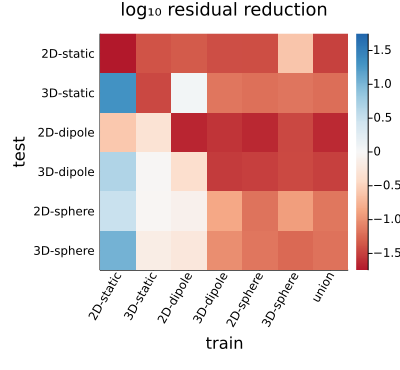
\includegraphics[width=\textwidth]{figures/crossloss.png}
        \caption{$\log_{10}$ residual reduction}
        \label{fig:cross plot}
    \end{subfigure}
    \hfill
    \begin{subfigure}[b]{0.47\textwidth}
        \centering
        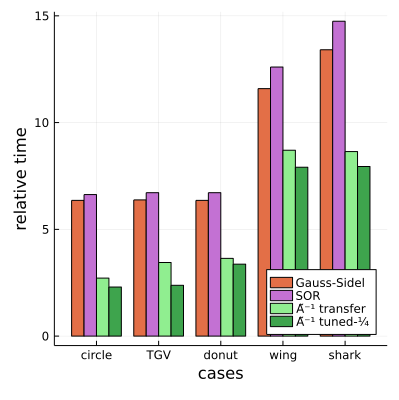
\includegraphics[width=\textwidth]{figures/crosscount.png}
        \caption{Solver time}
        \label{fig:synthetic time}
    \end{subfigure}
    \caption{(a-c) Sample solutions from the data-sets of three of the six synthetic cases. (d) Residual reduction over a single Multi-grid V-cycle on the `test' cases after tuning using the `train' case. Training case `union` refers to the smoother trained on all of the synthetic cases. (b) Time to reduce pressure residual by $10^{-3}$ for classical and parameterized smoothers on each synthetic case. Time is relative to the time of a single V-cycle using the Jacobi smoother.}
    \label{fig:synthetic cases}
\end{figure}



\section{Results}

\begin{figure}
    \centering
    \begin{subfigure}[b]{0.3\textwidth}
        \centering
        \caption{circle flow}
        \label{fig:circle}
    \end{subfigure}
    \begin{subfigure}[b]{0.3\textwidth}
        \centering
        \caption{Taylor-Green Vortex}
        \label{fig:TGV}
    \end{subfigure}
    \begin{subfigure}[b]{0.3\textwidth}
        \centering
        \caption{flapping wing}
        \label{fig:donut}
    \end{subfigure}
    \begin{minipage}{0.45\textwidth}
        \begin{subfigure}{\textwidth}
        \centering
        \caption{torus flow}
        \label{fig:donut}
        \end{subfigure}
        \begin{subfigure}{\textwidth}
        \centering
        \caption{swimming shark}
        \label{fig:donut}
        \end{subfigure}
    \end{minipage}
    \hfill
    \begin{subfigure}[b]{0.5\textwidth}
        \centering
        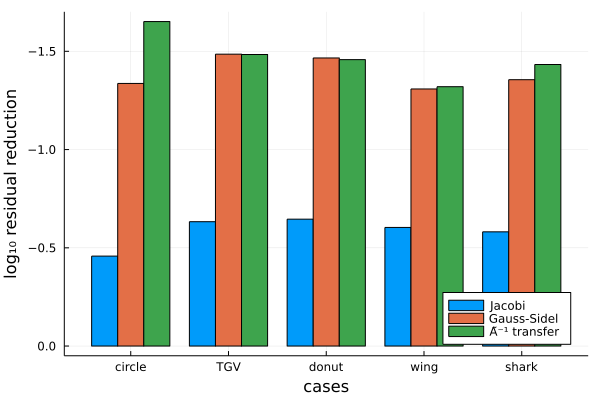
\includegraphics[width=\textwidth]{figures/compareloss.png}
        \caption{$\log_{10}$ residual reduction}
        \label{fig:synthetic time}
    \end{subfigure}
    \caption{(a-e) Snapshots from the five flow simulation cases. The Taylor-Green Vortex and torus flow are 3D cases, and the flapping wing and swimming shark have dynamic geometries. (f) Residual reduction over a single Multi-grid V-cycle for classical and parameterized smoothers on each case. The `transfer' smoother has been trained on the union of the synthetic data sets from Figure~\ref{fig:synthetic cases}.}
    \label{fig:simulation cases}
\end{figure}

\begin{figure}
    \centering
    \begin{subfigure}[b]{0.48\textwidth}
        \centering
        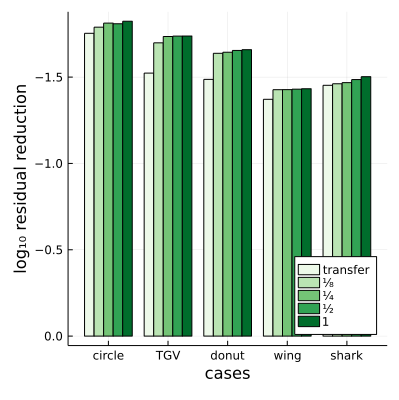
\includegraphics[width=\textwidth]{figures/scaleloss.png}
        \caption{$\log_{10}$ residual reduction}
        \label{fig:scaled loss}
    \end{subfigure}
    \hfill
    \begin{subfigure}[b]{0.48\textwidth}
        \centering
        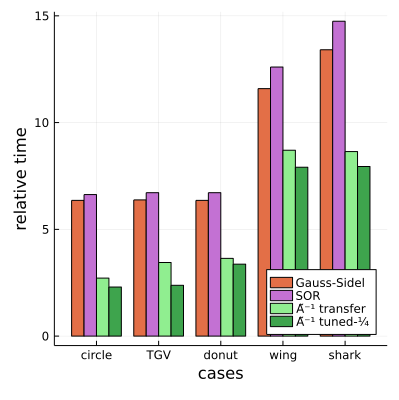
\includegraphics[width=\textwidth]{figures/crosscount.png}
        \caption{Solver time}
        \label{fig:simulation time}
    \end{subfigure}
        \caption{(a) Residual reduction over a single Multi-grid V-cycle on the full-resolution case. The `transfer' smoother has been trained on the union of the synthetic data sets from Figure~\ref{fig:synthetic cases}. The $\frac 18, \frac 14, \frac 12$ smoothers have been trained on simulations with the indicated reduced resolution \textit{in each spacial and temporal dimension}. (b) Time to reduce pressure residual by $10^{-3}$ for classical and parameterized smoothers on each simulation case. Time is relative to the time of a single V-cycle using the Jacobi smoother.}
        \label{fig:tuned simulation}
\end{figure}


\section{Conclusions}

\section*{References}

\bibliography{mybibfile}

\end{document}